%!TEX root = ../main.tex

\subsection{Geometric component}
\label{ss:geometric_component}
	Let us emphasize again that only a single primitve, i.e. three vertices and their associated normals, is used for the construction of the geometric and normal component. The vertices contain the three-dimensional vertex location together with a shared normal per vertex, i.e., the normal of each vertex is the same for every primitive using that vertex. \Cref{fig:method:input_primitive} shows an illustration of an input primitive, based on such input primitives the geometric component of the point-normal triangle is constructed.

	\begin{figure}
		\centering
		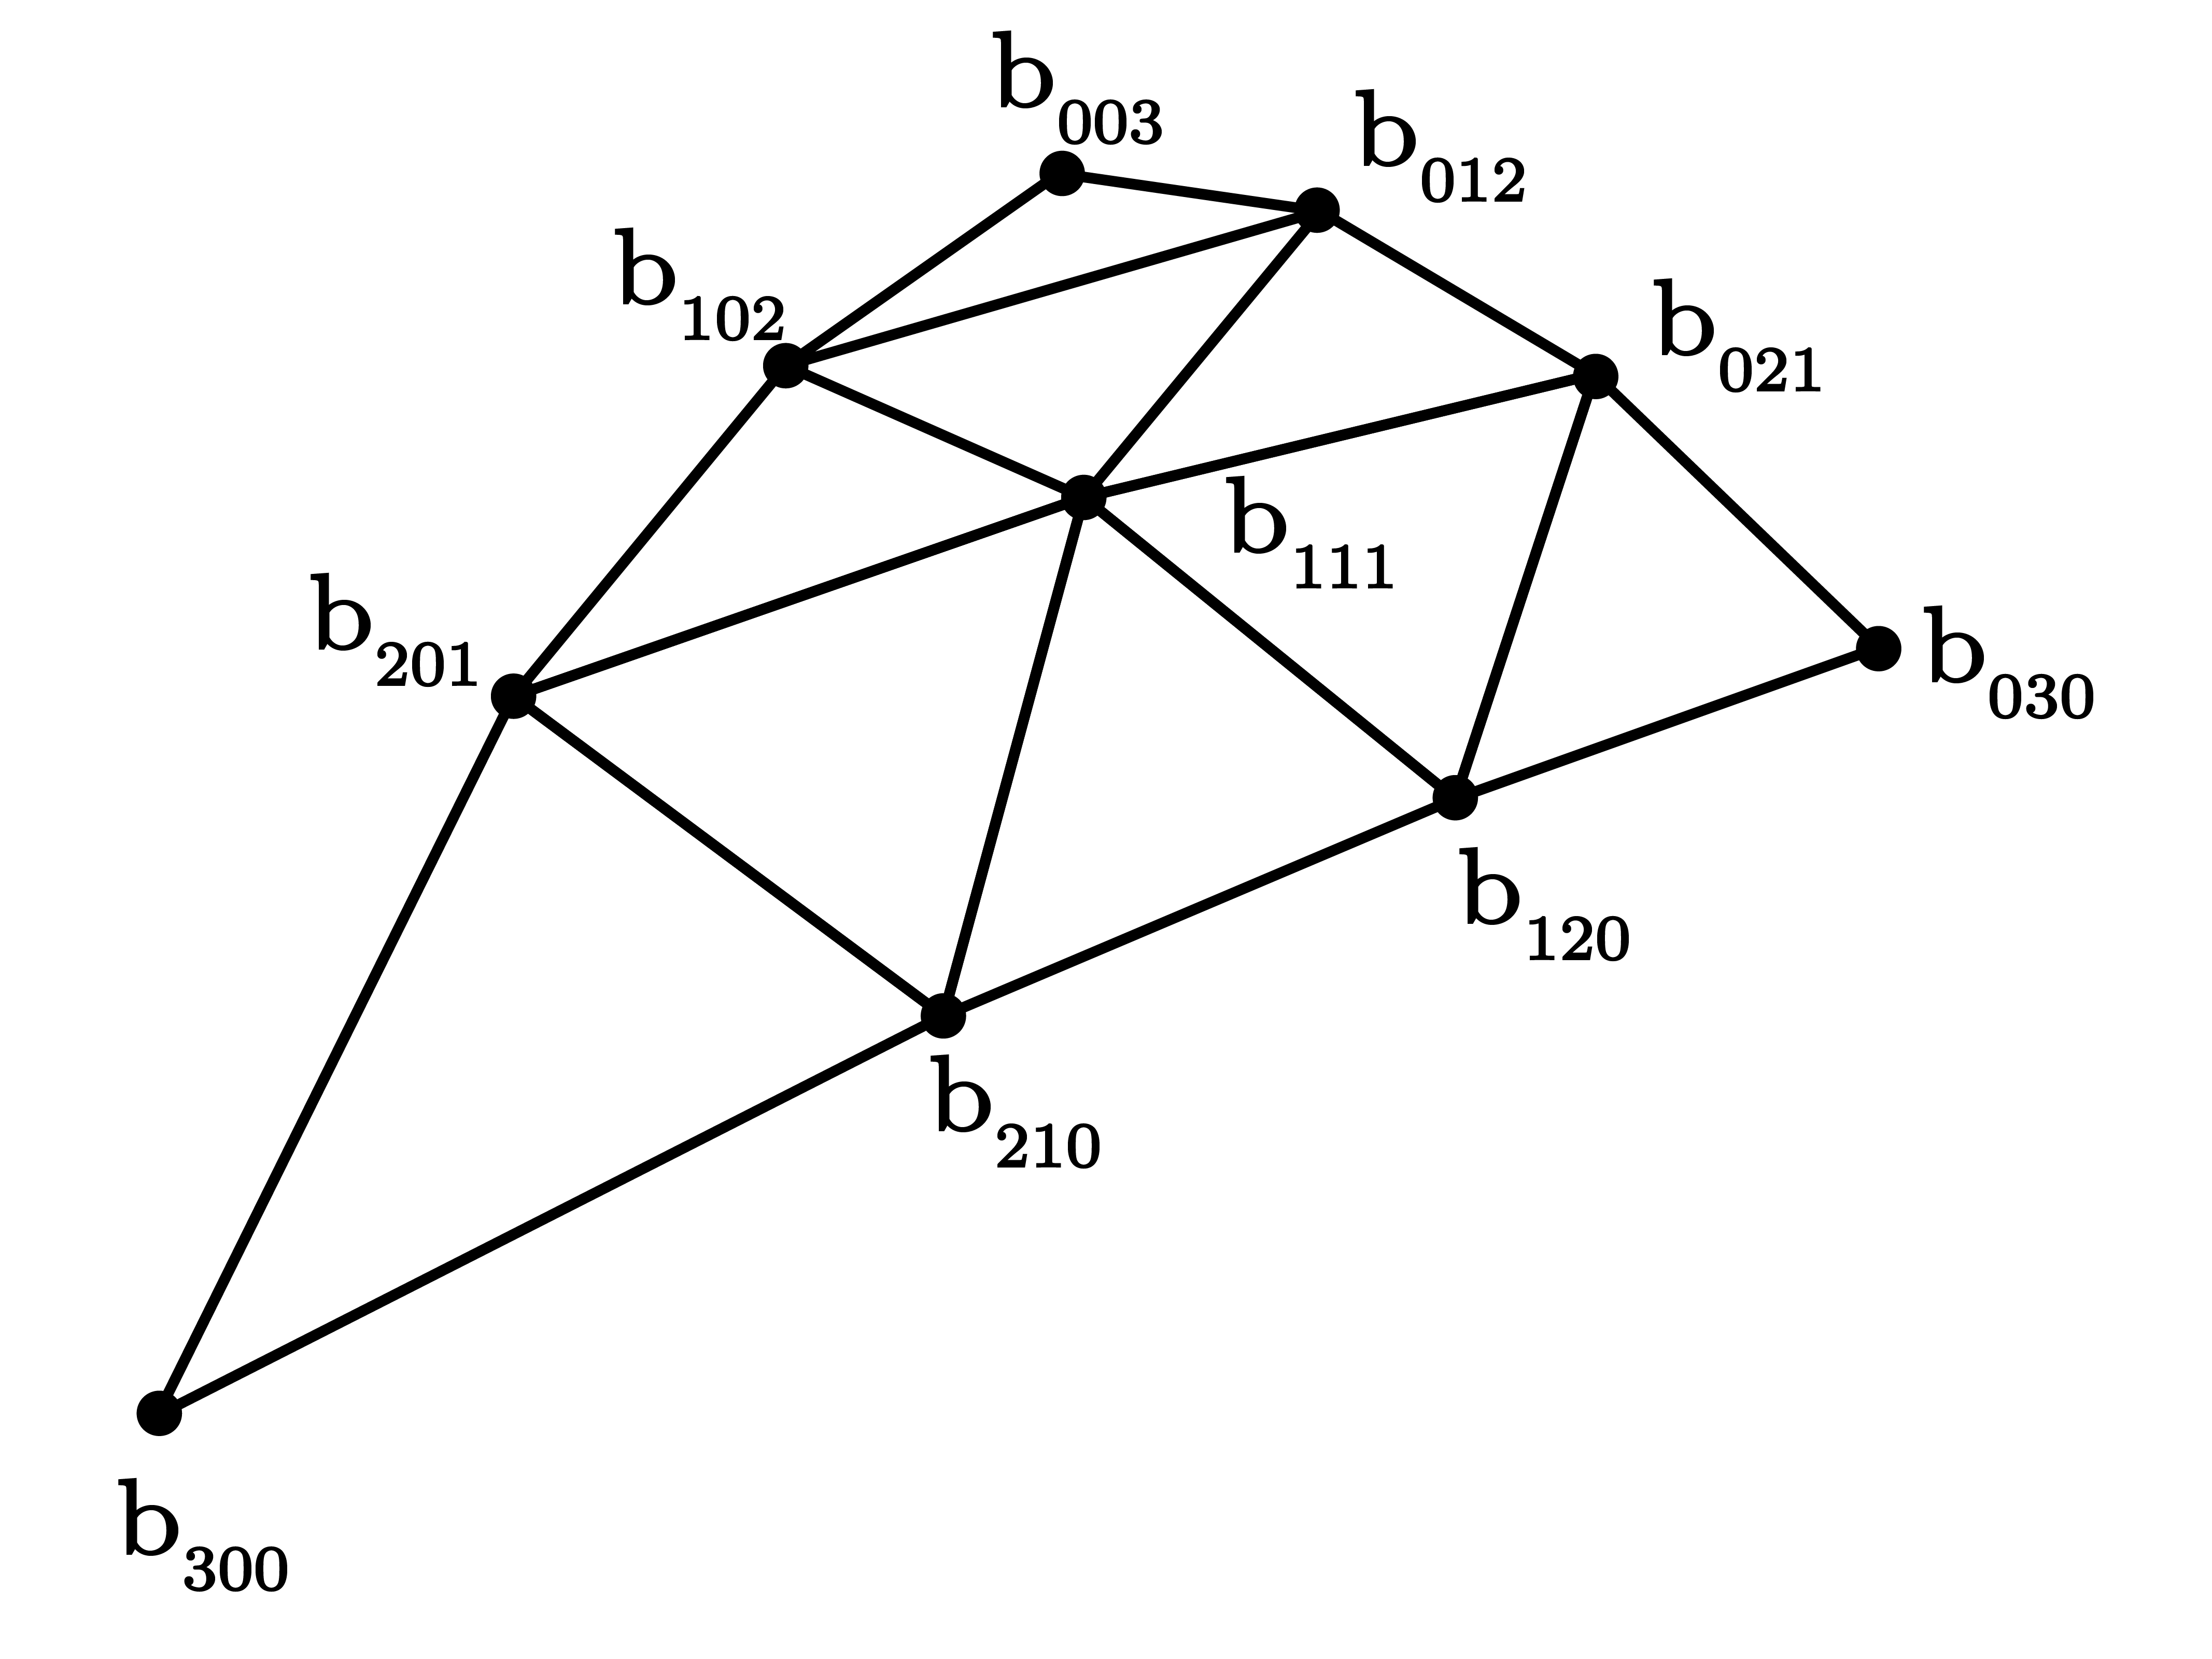
\includegraphics[width=0.45\textwidth]{./content/img/method/geometry_component.png}
		\caption{The geometric component of a point-normal triangle, i.e. the control net of a cubic Bézier triangle.}
		\label{fig:method:control_net}
	\end{figure}
	% ## Geometric component defined by triangluar cubic Bezier patch.
	%
	In the next section we discuss the definition of the geometry of a point-normal triangle. In \crefs{sss:method:geometry:construction} we discuss the construction of the control points that define the geometry. \Crefs{sss:method:geometry:properties} reviews the properties of the geometric component of a point-normal triangle.

\subsubsection{Basic form}
\label{sss:method:geometry:basicForm}
	The geometric component of a point-normal triangle is defined as a triangular cubic Bézier patch. Such a patch $b(u,v)$ is defined as follows:
	%
	\begin{align}
	\noalign{$b(u,v): \quad R^2 \mapsto R^3,\quad$ for $w = 1 - u - v, \quad u, v, w \geq 0$}
	\begin{split}\label{eq:method:cubic_bezier_patch}
	    b(u,v) ={}& \sum_{i + j + k = 3} b_{ijk}\frac{3!}{i!j!k!} u^i v^j w^k\\
	      	   ={}& b_{300}w^3 + b_{030}u^3 + b_{003}v^3\\
	      	    {}& + b_{210}3w^3 + b_{120}3wu^2 + b_{201}3w^2v\\
	      	    {}& + b_{021}3u^2v + b_{102}2wv^2 + b_{012}3uv^2\\
	      	    {}& + b_{111}6wuv.
	\end{split}
	\end{align}
	%
	The $b_{ijk}$ parameters in \crefe{eq:method:cubic_bezier_patch} are the control points of the patch, also called coefficients. In \cref{fig:method:control_net} the visualization of the network of these control points is shown. We distinguish three different groups of control points, each with their own method of construction: 
	%
	\begin{align*}
		\text{vertex coefficients: } {}&  b_{300},\ b_{030},\ b_{003} \\
		\text{tangent coefficients: } {}&  b_{210},\ b_{120},\ b_{021},\ b_{012},\ b_{102},\ b_{201}\\
		\text{center coefficient: }   {}&  b_{111}
	\end{align*}

	\Crefe{eq:method:cubic_bezier_patch} can be used to evaluate any point on the patch that is parameterized by the barycentric coordinates $(u,v,w)$. This evaluation is done in the triangulation stage of the rendering process. In this stage the cubic Bézier surface is approximated by using a number of smaller flat triangles; these are eventually rendered. The number of sub-triangles is determined by the level of detail (lod). For the original sub-triangulation scheme we refer the reader to \textcite{vlachos2001curved}, as this is where the implementation presented in this paper deviates from the one discussed by \citeauthor{vlachos2001curved}. For a more exhaustive discussion of these differences we refer the reader to \crefs{s:implementation}.

	As stated above the geometry of a point-normal triangle is a cubic Bézier patch. This degree of patches is a trade-off between simplicity, visual performance, and computational cost. Quadratic patches do not provide the same modeling range of a surface as a cubic patch \cite{boubekeur2008phong}. For example, a cubic representation is necessary to capture inflections implied by the triangle position and normal data. \citeauthor{vlachos2001curved} state that there is no additional data to suggest a higher degree is needed, and that therefore they settled on the form of $b(u,v)$ as presented in \crefe{eq:method:cubic_bezier_patch}.

\subsubsection{Coefficients} 
\label{sss:method:geometry:construction}
	This section discusses how the `curved' control net geometry, see \cref{fig:method:control_net}, is calculated from the flat input primitive shown in \cref{fig:method:input_primitive}. The input primitive provides the positions $P_1, P_2, P_3 \in \Real^3$ and normals $N_1, N_2, N_3 \in \Real^3$. The coefficients $b_{ijk}$ are computed as follows:
	%
	\begin{enumerate}[label=(\roman*)]
		\item 
			Initially, the coefficients $b_{ijk}$ are spread uniformly, i.e., the intermediate position of $b_{ijk}$ is calculated according to
			\begin{align*}
				b_{ijk} = \frac{(i P_1 + j P_2 + k P_3)}{3}.
			\end{align*}
		\item 
			The intermediate positions of the vertex coefficients are the same as their final positions, see \crefe{eq:method:vertex_coefficients}. Their intermediate position places them at the vertices of the input triangle, and this is where they are required to stay to keep the mesh watertight.
		\item 
			The tangent coefficients are placed at their final position by projecting the intermediate position into the tangent plane of the closest corner, see \crefe{eq:method:tangent_coefficients}. This step is illustrated in \cref{fig:method:geometry_tangent_projection.png}.
		\item The center coefficient is moved to the average of the tangent coefficients plus \rfrac{1}{2} times the distance it had to travel from its intermediate position, see \crefe{eq:method:center_coefficient}.
	\end{enumerate}
	%
	\begin{figure}
		\centering
		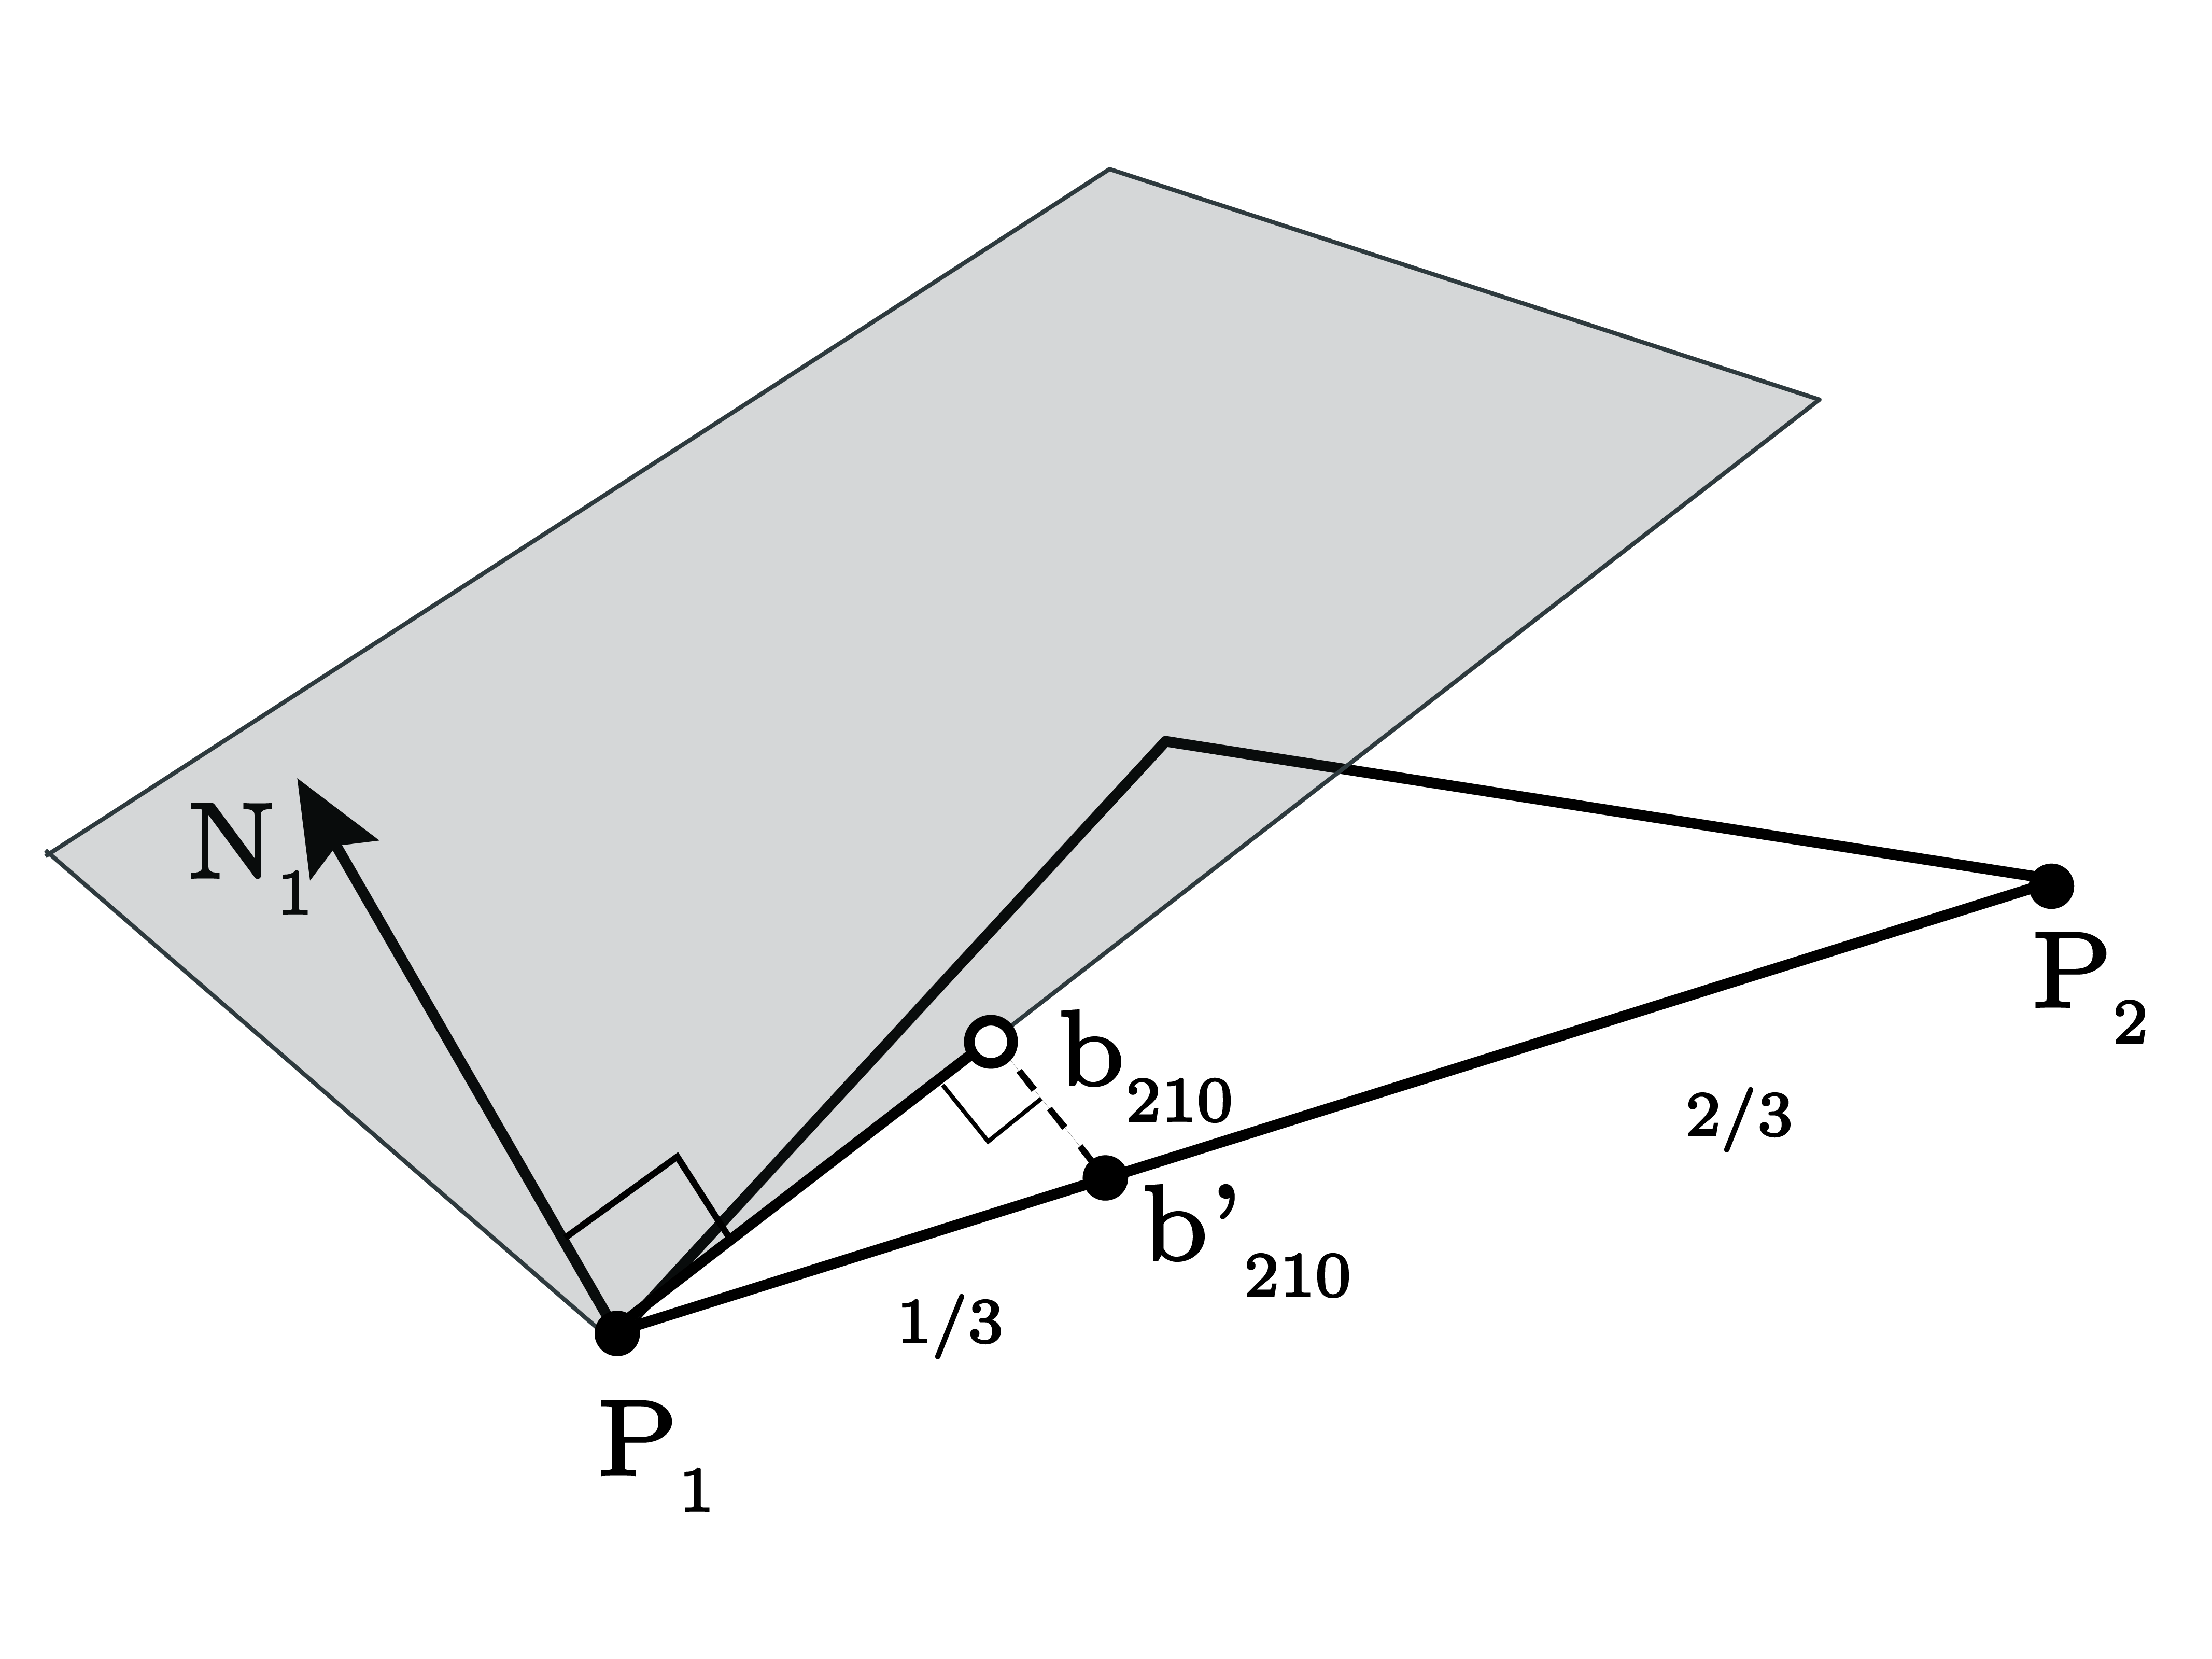
\includegraphics[width=0.45\textwidth]{./content/img/method/geometry_computation.png}
		\caption{Projection of the initial tangent coefficient $b_{210}'$ to the tangent plane of the closest vertex $P_1$, which results in the final tangent coefficient $b_{210}$. The initial position is represented with a filled circle, the final position with the outline of a circle. Illustration adapted from \textcite{vlachos2001curved}.}
		\label{fig:method:geometry_tangent_projection.png}
	\end{figure}

	The following set of formulas describe how the positions of the coefficients are calculated. For clarity, we group together the formulas in the same way as the coefficients. The \textit{vertex coefficients} are defined as:
	\begin{align}\label{eq:method:vertex_coefficients}
		b_{300} = P_1,\ b_{030} = P_2,\ b_{003} = P_3.
	\end{align}

	The tangent coefficients are given by the projection of a point $Q$ onto the plane defined by the normal $N$ of the point $P$. The projected point $Q'$ is then given by: $Q' = Q - wN$, where $w = (Q - P) \cdot N$. Using this the positions of the \textit{tangent coefficients} are defined as:
	\begin{equation}\label{eq:method:tangent_coefficients}
		\begin{aligned}
			b_{210} = {}& (2 P_1 + P_2 - w_{12}N_1) / 3,\\
			b_{120} = {}& (2 P_2 + P_1 - w_{21}N_2) / 3,\\
			b_{021} = {}& (2 P_2 + P_3 - w_{23}N_2) / 3,\\
			b_{012} = {}& (2 P_3 + P_2 - w_{32}N_3) / 3,\\
			b_{102} = {}& (2 P_3 + P_1 - w_{31}N_3) / 3,\\
			b_{201} = {}& (2 P_1 + P_3 - w_{13}N_1) / 3, 
		\end{aligned}		
	\end{equation}
	where
	\begin{equation*}
		w_{ij} = (P_j - P_i) \cdot N_i \in \Real.
	\end{equation*}


	The center coefficient is, as stated before, moved to the average of the previous computed tangent coefficients plus $\rfrac{1}{2}$ times the distance it traveled from its intermediate location to that average position. The \textit{center coefficient}, is computed as:
	\begin{equation}\label{eq:method:center_coefficient}
		b_{111} = E + (E - V) / 2,
	\end{equation}
	where
	\begin{align*}
		E = {}& \frac{b_{210} + b_{120} + b_{021} + b_{012} + b_{102} + b_{201}}{6}\\
		V = {}& \frac{(P_1 + P_2 + P_3)}{3}.
	\end{align*}

	Combining \crefe{eq:method:vertex_coefficients} through \ref{eq:method:center_coefficient} computes the control net shown in \cref{fig:method:control_net}, based on the input primitive presented in \cref{fig:method:input_primitive}.

\subsubsection{Properties}
\label{sss:method:geometry:properties}
	\citeauthor{vlachos2001curved} have shown that point-normal triangles do not deviate too much from the original triangle. This is an important property since it ensures that the shape of the model is preserved and that adjacent triangles do not interfere with each other. 

	By demanding that normals are shared, i.e., one unique normal per vertex, the boundary between two point-normal triangles is generated with the same algorithm, consequently the surface is water tight. Except at the corners, PN triangles do not usually join with tangent continuity \cite{vlachos2001curved}. If the normals are not shared, cracks will form as illustrated in \cref{fig:method:cracks}.

	\begin{figure}
		\centering
		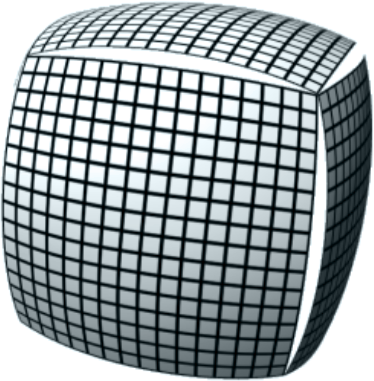
\includegraphics[width=0.4\columnwidth]{./content/img/method/cracks.png}
		\caption{An illustration of what would happen if one renders a model using point-normal triangles where vertices have different normals, depending on the associated faces. Image taken from \cite{mcdonald2010crack}.}
		\label{fig:method:cracks}
	\end{figure}
